\documentclass[onecolumn]{article}

%Titling
    \usepackage[compact]{titlesec}
    \titlespacing{\section}{0pt}{3ex}{2ex}
    \titlespacing{\subsection}{0pt}{2ex}{1ex}
    \titlespacing{\subsubsection}{0pt}{1ex}{0.5ex}
\titleformat*{\section}{\Large\scshape}
\titleformat*{\subsection}{\Large}
\titleformat{\subsubsection}[runin]
  {\normalfont\bfseries}{\thesubsection}{1em}{}
  
%Page size
	\addtolength{\oddsidemargin}{-.875in}
	\addtolength{\evensidemargin}{-.875in}
	\addtolength{\textwidth}{1.75in}

	\addtolength{\topmargin}{-.875in}
	\addtolength{\textheight}{1.75in}
	
	\parskip=.1cm
	
%Indented paragraph
\setlength{\parindent}{0pt}
\newenvironment{indentpar}[1]
  {\begin{list}{}
          {\setlength{\rightmargin}{#1}}
          \item[]
  }
  {\end{list}}

% tikz setup
\usepackage{tikz}
\usetikzlibrary{shapes,arrows}
\newcommand*{\h}{\hspace{5pt}}% for indentation
\newcommand*{\hh}{\h\h}% double indentation

\begin{document}

% Missing -> MIMIC
\begin{figure}
\centering
  % setting the typeface to sans serif and the font size to small
  % the scope local to the environment
  \sffamily
  \footnotesize
  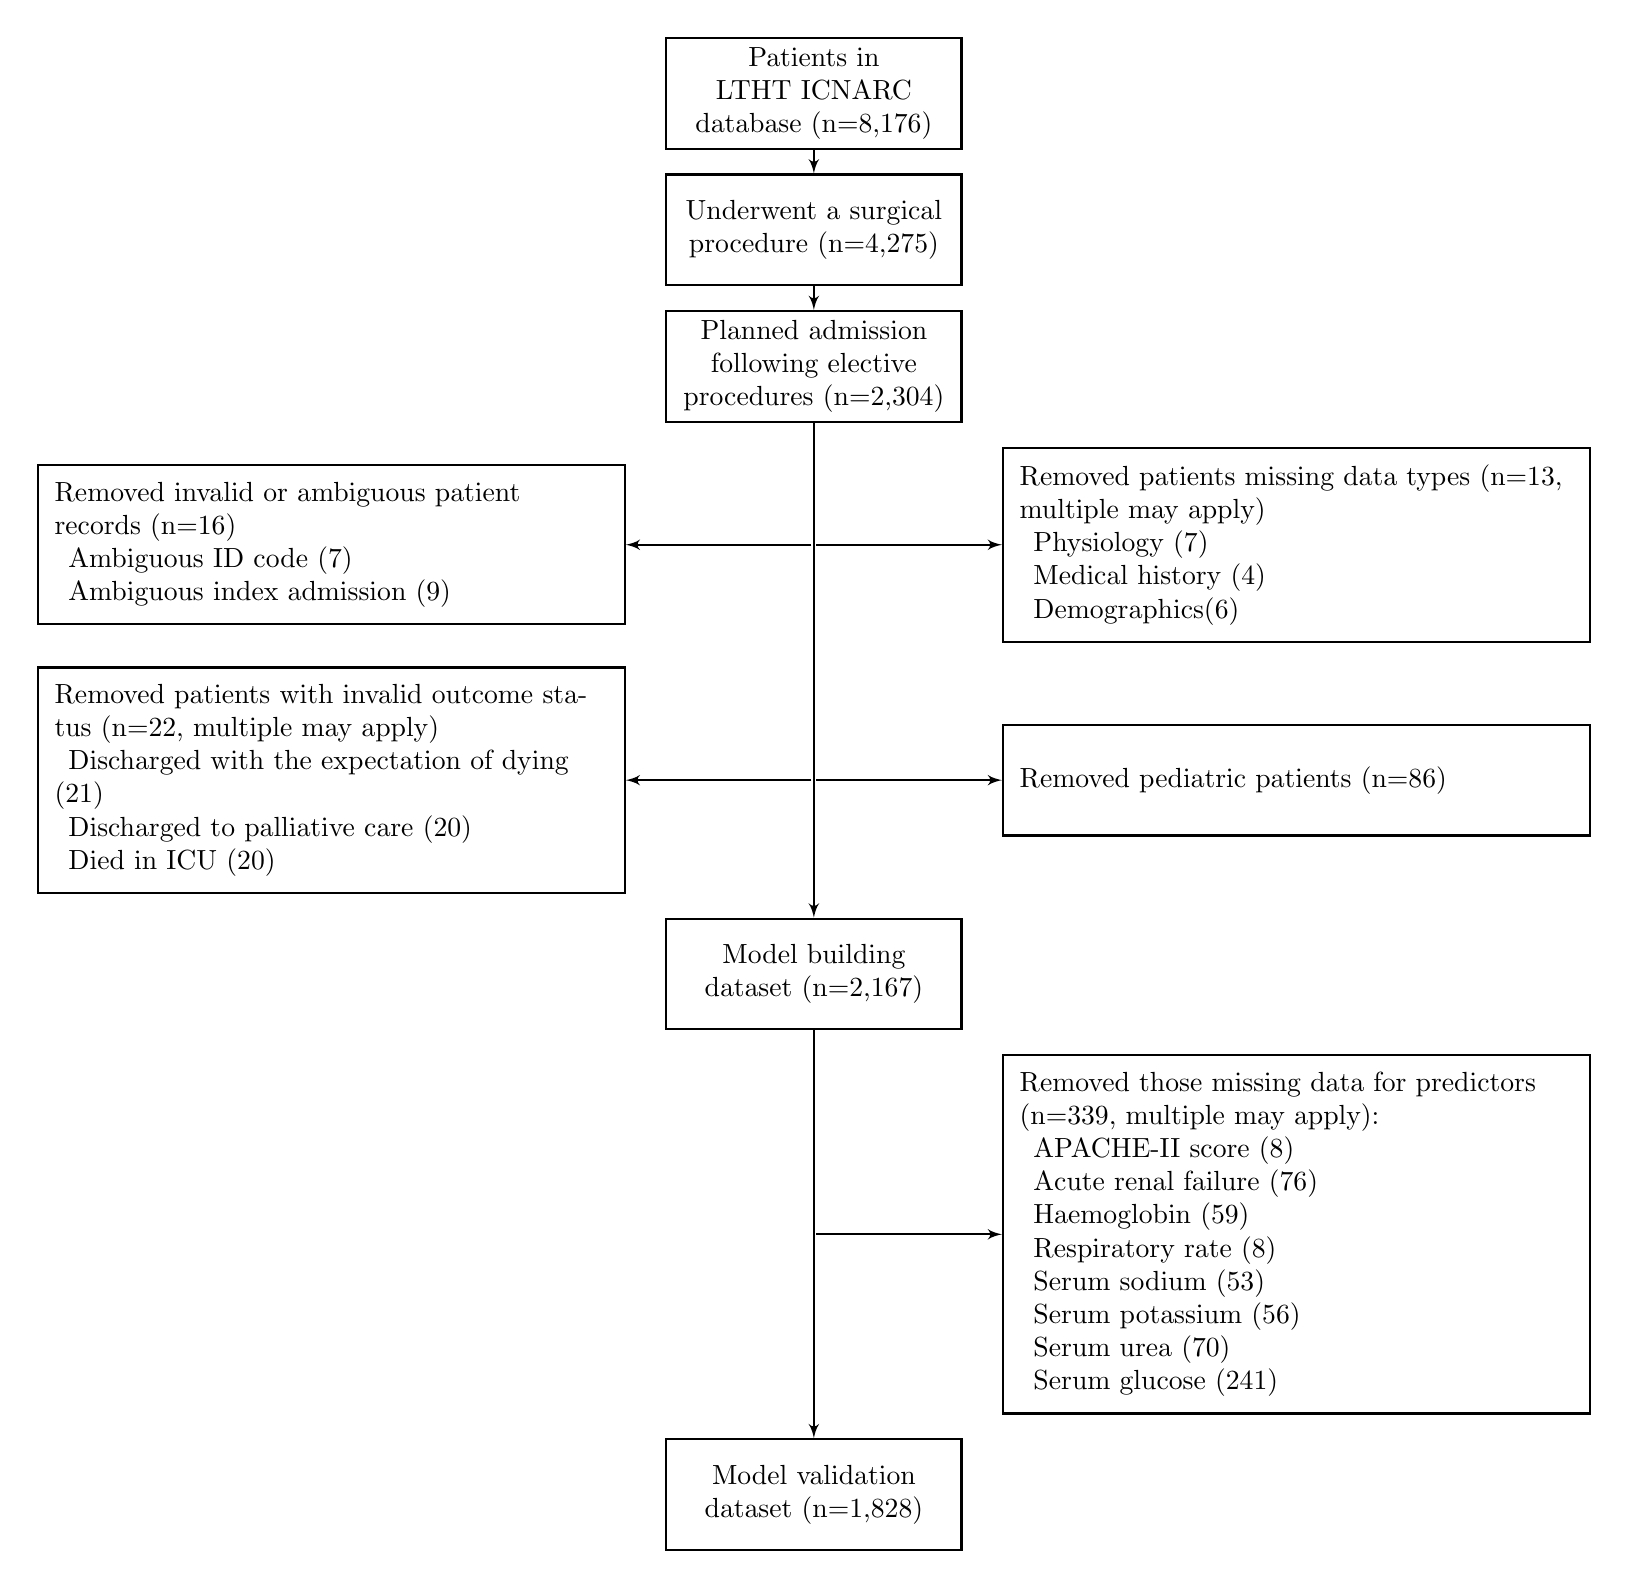
\begin{tikzpicture}[auto,
    block_center/.style ={rectangle, draw=black, thick, fill=white,
      text width=10em, text centered,
      minimum height=4em},
    block_left/.style ={rectangle, draw=black, thick, fill=white,
      text width=20em, text ragged, minimum height=4em, inner sep=6pt},
      line/.style ={draw, thick, -latex', shorten >=0pt},
          block_noborder/.style ={rectangle, draw=none, thick, fill=none,
      text width=-4em, text centered, minimum height=1em}]
    % outlining the flowchart using the PGF/TikZ matrix funtion
    \matrix [column sep=5mm,row sep=3mm] {
      % row 1
      & \node [block_center] (full) {Patients in LTHT ICNARC database (n=8,176)};\\
      % row 2
      &\node [block_center] (service) {Underwent a surgical procedure (n=4,275)}; \\
      % row 3
      &\node [block_center] (elective) {Planned admission following elective procedures (n=2,304)};\\
      % row 4
              \node [block_left] (invalid) {Removed invalid or ambiguous patient records (n=16)\\
              \h Ambiguous ID code (7)\\
              \h Ambiguous index admission (9)};
            & \node [block_noborder] (hidden_r4) {};&     
      \node [block_left] (missingtypes) {Removed patients missing data types (n=13, multiple may apply)\\
      \h Physiology (7)\\
      \h Medical history (4)\\
      \h Demographics(6)}; \\
      % row 5
       \node [block_left] (dead) {Removed patients with invalid outcome status (n=22, multiple may apply)\\
              \h Discharged with the expectation of dying (21)\\
              \h Discharged to palliative care (20)\\
              \h Died in ICU (20)};
            & \node [block_noborder] (hidden_r5) {};&     
      \node [block_left] (pediatric) {Removed pediatric patients (n=86)}; \\
               &
       \node [block_center] (building) {Model building dataset (n=2,167)};& \\  
      % row 7
      &
           \node [block_noborder] (hidden_r6) {};&
      \node [block_left] (missing) {Removed those missing data for predictors (n=339, multiple may apply): \\
		\h APACHE-II score (8)\\
		\h Acute renal failure (76)\\
		\h Haemoglobin (59)\\
		\h Respiratory rate (8)\\
		\h Serum sodium (53)\\
		\h Serum potassium (56)\\
		\h Serum urea (70)\\
		\h Serum glucose (241)
        }; \\  
        % row 8  
       &
       \node [block_center] (final) {Model validation dataset (n=1,828)};& \\  
      };
    % end matrix
     connecting nodes with paths
    \begin{scope}[every path/.style=line]
     \path (full)   -- (service);
     \path (service)   -- (elective);
     \path (elective)   -- (building);
     \path (hidden_r4)   -- (invalid);
     \path (hidden_r4)   -- (missingtypes);
     \path (hidden_r5)   -- (pediatric);
     \path (hidden_r5)   -- (dead);
     \path (building)   -- (final);
     \path (hidden_r6)   -- (missing);
    \end{scope}  
  \end{tikzpicture}
\end{figure}

% Readmission -> ICNARC
\begin{figure}
\centering
  % setting the typeface to sans serif and the font size to small
  % the scope local to the environment
  \sffamily
  \footnotesize
  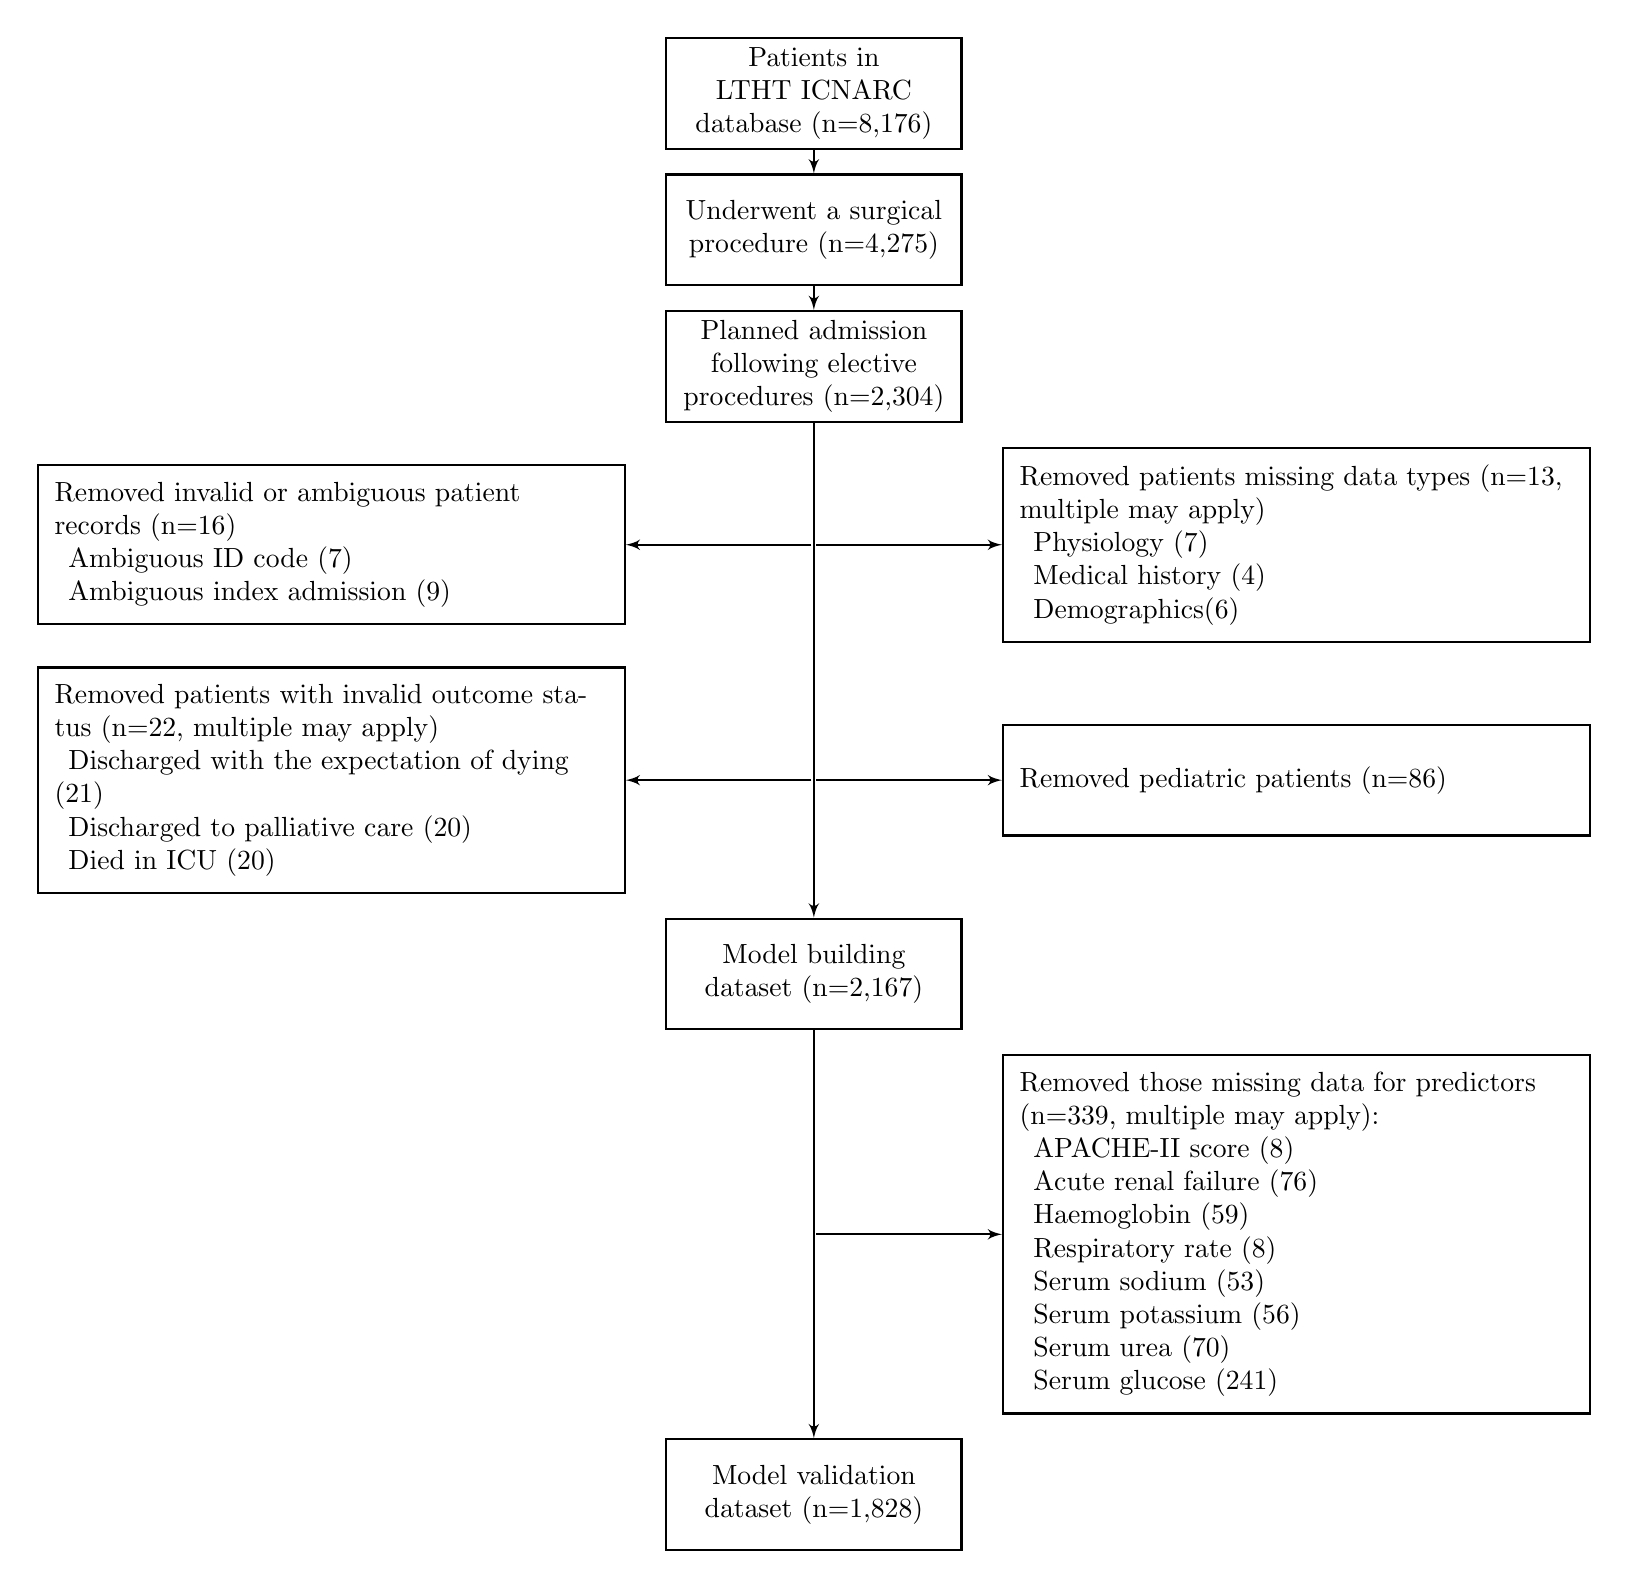
\begin{tikzpicture}[auto,
    block_center/.style ={rectangle, draw=black, thick, fill=white,
      text width=10em, text centered,
      minimum height=4em},
    block_left/.style ={rectangle, draw=black, thick, fill=white,
      text width=20em, text ragged, minimum height=4em, inner sep=6pt},
      line/.style ={draw, thick, -latex', shorten >=0pt},
          block_noborder/.style ={rectangle, draw=none, thick, fill=none,
      text width=-4em, text centered, minimum height=1em}]
    % outlining the flowchart using the PGF/TikZ matrix funtion
    \matrix [column sep=5mm,row sep=3mm] {
      % row 1
      & \node [block_center] (full) {Patients in LTHT ICNARC database (n=8,176)};\\
      % row 2
      &\node [block_center] (service) {Underwent a surgical procedure (n=4,275)}; \\
      % row 3
      &\node [block_center] (elective) {Planned admission following elective procedures (n=2,304)};\\
      % row 4
              \node [block_left] (invalid) {Removed invalid or ambiguous patient records (n=16)\\
              \h Ambiguous ID code (7)\\
              \h Ambiguous index admission (9)};
            & \node [block_noborder] (hidden_r4) {};&     
      \node [block_left] (missingtypes) {Removed patients missing data types (n=13, multiple may apply)\\
      \h Physiology (7)\\
      \h Medical history (4)\\
      \h Demographics(6)}; \\
      % row 5
       \node [block_left] (dead) {Removed patients with invalid outcome status (n=22, multiple may apply)\\
              \h Discharged with the expectation of dying (21)\\
              \h Discharged to palliative care (20)\\
              \h Died in ICU (20)};
            & \node [block_noborder] (hidden_r5) {};&     
      \node [block_left] (pediatric) {Removed pediatric patients (n=86)}; \\
               &
       \node [block_center] (building) {Model building dataset (n=2,167)};& \\  
      % row 7
      &
           \node [block_noborder] (hidden_r6) {};&
      \node [block_left] (missing) {Removed those missing data for predictors (n=339, multiple may apply): \\
		\h APACHE-II score (8)\\
		\h Acute renal failure (76)\\
		\h Haemoglobin (59)\\
		\h Respiratory rate (8)\\
		\h Serum sodium (53)\\
		\h Serum potassium (56)\\
		\h Serum urea (70)\\
		\h Serum glucose (241)
        }; \\  
        % row 8  
       &
       \node [block_center] (final) {Model validation dataset (n=1,828)};& \\  
      };
    % end matrix
     connecting nodes with paths
    \begin{scope}[every path/.style=line]
     \path (full)   -- (service);
     \path (service)   -- (elective);
     \path (elective)   -- (building);
     \path (hidden_r4)   -- (invalid);
     \path (hidden_r4)   -- (missingtypes);
     \path (hidden_r5)   -- (pediatric);
     \path (hidden_r5)   -- (dead);
     \path (building)   -- (final);
     \path (hidden_r6)   -- (missing);
    \end{scope}  
  \end{tikzpicture}
\end{figure}

% Readmission -> MIMIC
\begin{figure}
\centering
  % setting the typeface to sans serif and the font size to small
  % the scope local to the environment
  \sffamily
  \footnotesize
  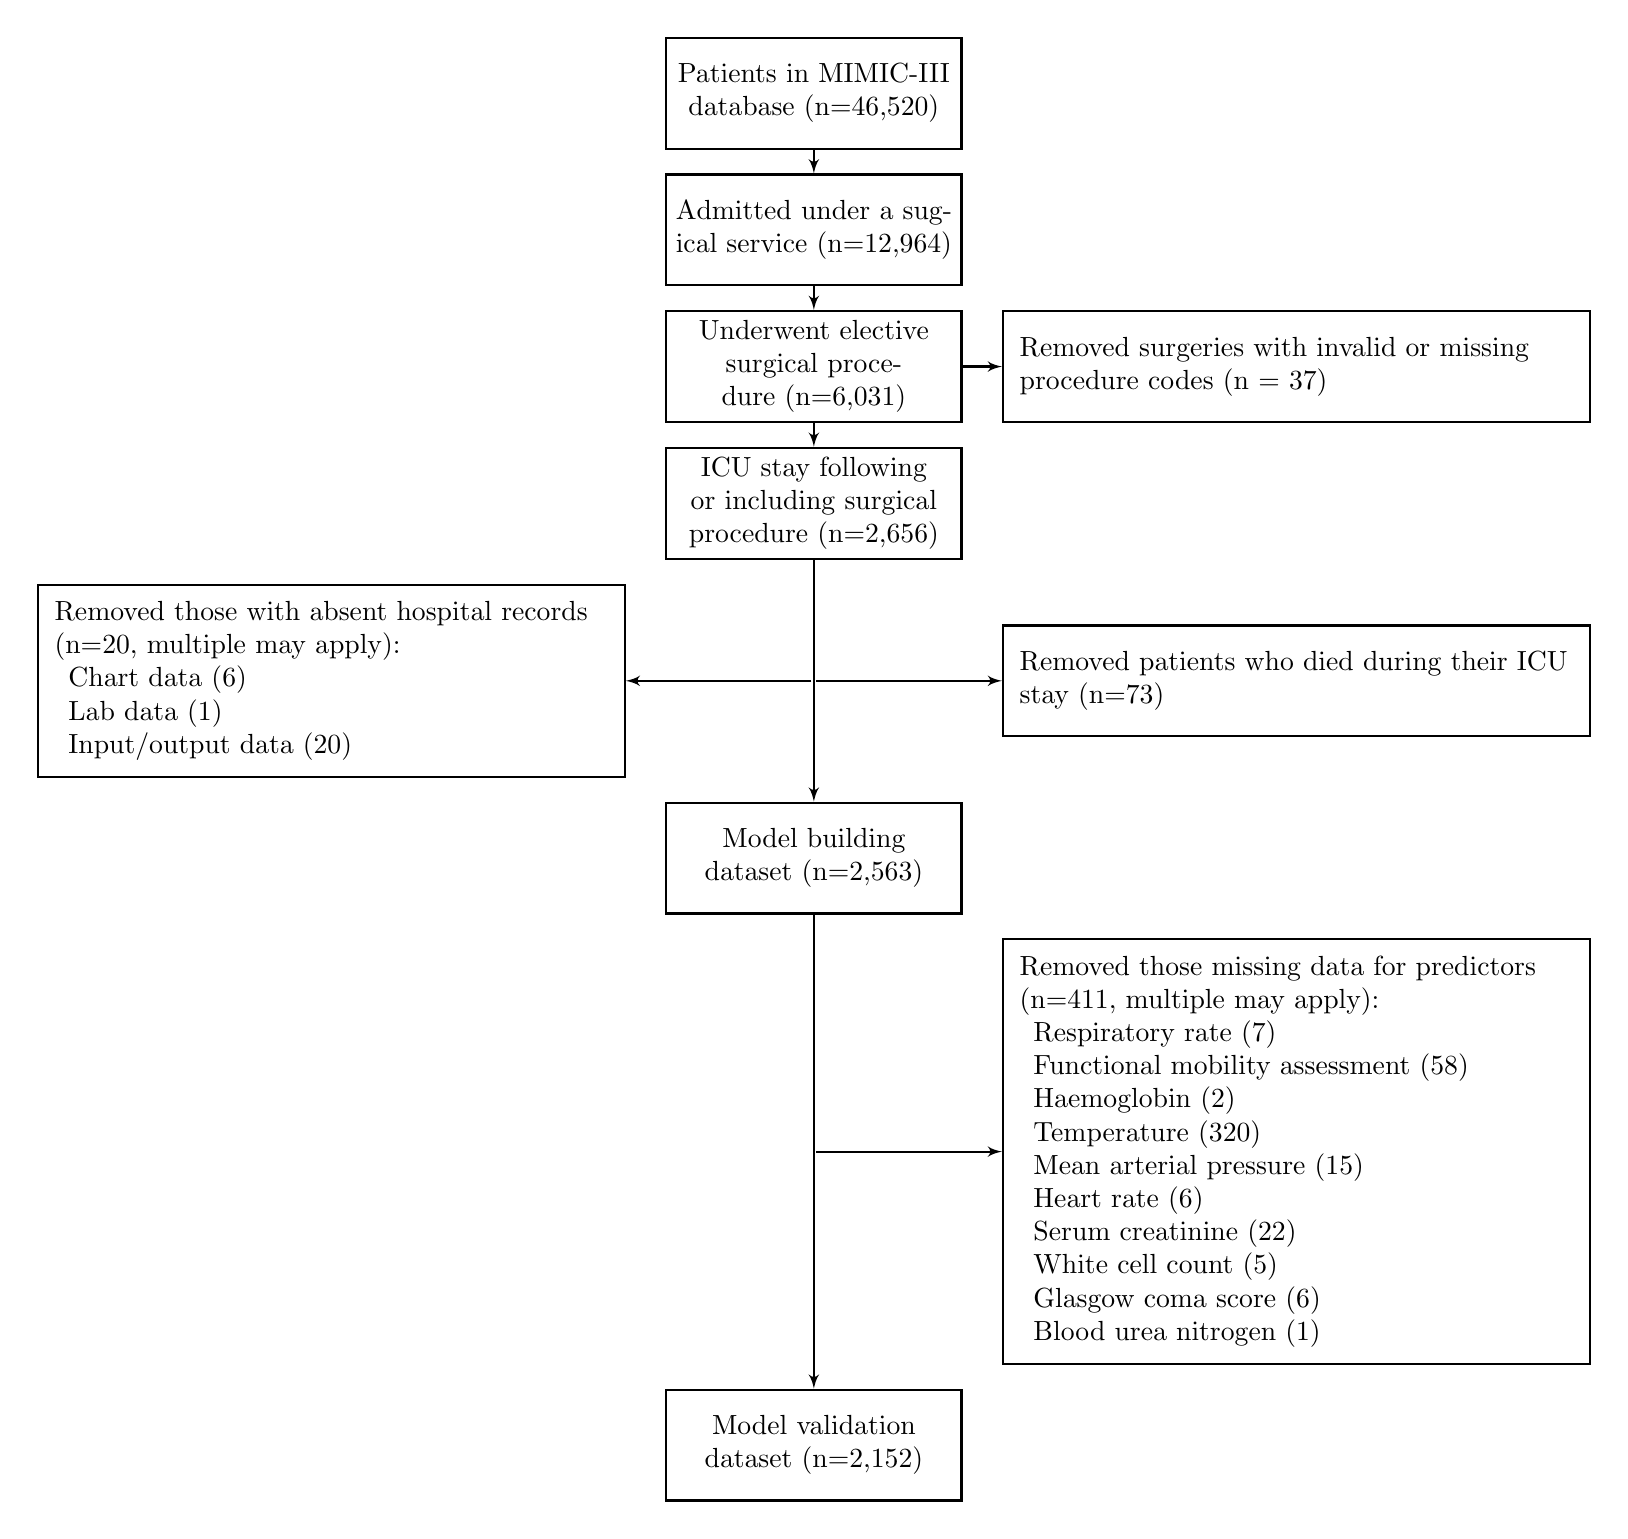
\begin{tikzpicture}[auto,
    block_center/.style ={rectangle, draw=black, thick, fill=white,
      text width=10em, text centered,
      minimum height=4em},
    block_left/.style ={rectangle, draw=black, thick, fill=white,
      text width=20em, text ragged, minimum height=4em, inner sep=6pt},
      line/.style ={draw, thick, -latex', shorten >=0pt},
          block_noborder/.style ={rectangle, draw=none, thick, fill=none,
      text width=-4em, text centered, minimum height=1em}]
    % outlining the flowchart using the PGF/TikZ matrix funtion
    \matrix [column sep=5mm,row sep=3mm] {
      % row 1
      & \node [block_center] (full) {Patients in MIMIC-III database (n=46,520)};\\
      % row 2
      &\node [block_center] (service) {Admitted under a sugical service (n=12,964)}; \\
      % row 3
      &\node [block_center] (elective) {Underwent elective surgical procedure (n=6,031)};       
      & \node [block_left] (invalidprocedure) {Removed surgeries with invalid or missing procedure codes (n = 37)}; \\
      % row 4
        &\node [block_center] (icuprocedure) {ICU stay following or including surgical procedure (n=2,656)}; \\
      % row 5  
      \node [block_left] (nochart) {Removed those with absent hospital records (n=20, multiple may apply): \\
		\h Chart data (6)\\
	 	\h Lab data (1)\\
		\h Input/output data (20)
        };   &
       \node [block_noborder] (hidden_r5) {};&
               \node [block_left] (died) {Removed patients who died during their ICU stay (n=73)}; \\
        % row 6 
               &
       \node [block_center] (building) {Model building dataset (n=2,563)};& \\  
      % row 7
        &
           \node [block_noborder] (hidden_r6) {};&
      \node [block_left] (missing) {Removed those missing data for predictors (n=411, multiple may apply): \\
		\h Respiratory rate (7)\\
		\h Functional mobility assessment (58)\\
		\h Haemoglobin (2)\\
		\h Temperature (320)\\
		\h Mean arterial pressure (15)\\
		\h Heart rate (6)\\
		\h Serum creatinine (22)\\
		\h White cell count (5)\\
		\h Glasgow coma score (6)\\
		\h Blood urea nitrogen (1)
        }; \\  
        % row 8  
       &
       \node [block_center] (final) {Model validation dataset (n=2,152)};& \\  
      };
    % end matrix
     connecting nodes with paths
    \begin{scope}[every path/.style=line]
     \path (full)   -- (service);
      \path (service) -- (elective);
      \path (elective) -- (icuprocedure);
      \path (elective) -- (invalidprocedure);
      \path (hidden_r5) -- (died);
      \path (icuprocedure) -- (building);
      \path (building) -- (final);
      \path (hidden_r6) -- (missing);
      \path (hidden_r5) -- (nochart);
    \end{scope}  
  \end{tikzpicture}
\end{figure}
\end{document}
